\epart{Safety engineering}

\question{13}

An  \emph{implantable cardioverter-defibrillator}  is a device implanted in a person's chest that provides an electric shock when abnormal heart beats are detected; for example, in the case of the heart stopping beating, a large shock is delivered to re-start the heart.

Figure~\ref{fig:icd-loop} shows a system architecture for an \emph{implantable cardioverter-defibrillator} (ICD). The system is a closed-loop. The heart rate is read by the heart rate monitors, and this value is sent to the control unit. The software calculations inside the control unit decide what level of shock to deliver. If the level is non-zero, the small impulse generator is used to provide the shock to the heart. 
Note that there are three redundant heart-rate monitors operating in parallel, to mitigate the problem of faulty heart-rate monitors. In this system, the heart-rate monitors each provide a single reading to the ICD component, which uses approximate agreement majority voting to calculate a value for the heart rate. There is only one impulse generator, and one ICD control unit.

\begin{figure}[!h]
\centering
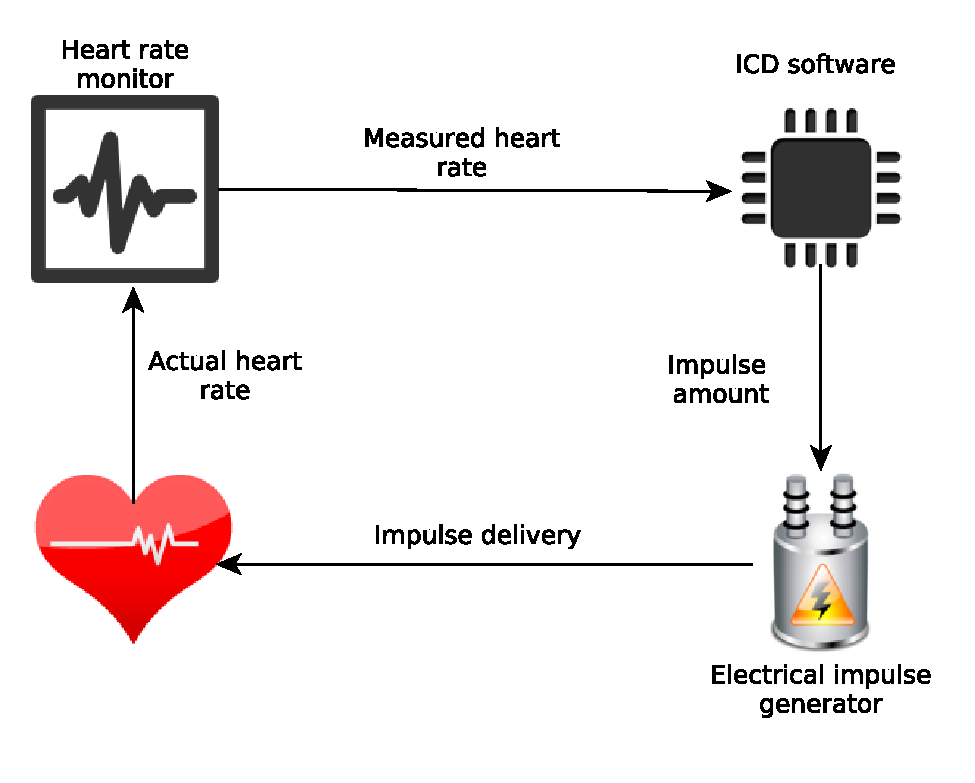
\includegraphics[scale=0.6]{./figs/icd-loop}
\caption{A model of the ICD system architecture.}
\label{fig:icd-loop}
\end{figure}


\subsubsection*{Safety conditions}

The following safety condition must be met by the ICD system:

\begin{quote}

 If the patient's heart is beating in a regular manner, they shall receive no shocks from the impulse generator.

\end{quote}

If this safety concern is violated, a hazard occurs.

Perform a fault tree analysis on the ICD software component for this hazard for the case when the heart receives a large joule shock. Your fault tree should outlines how the failure can occur, caused by the ICD software only. Briefly justify each choice that you make in your analysis, stating why you believe each level is \emph{necessary} or \emph{sufficient}.

The top-level event for the fault tree is the case in which the heart is shocked while having a regular heartbeat.

For this question, assume that the ICD software has the following functions:

 \begin{itemize}
  \item Receive the three heart rate readings (assume that heart rate monitors are functioning correctly).
  \item Vote on the three readings using an approximate agreement majority voting algorithm.
  \item Calculate the heart status: fibrillation (heart attack), tachycardia (increased, abnormal heartbeat), or normal. Fibrillation is when the standard deviation of the five previous readings is above a certain threshold.
  \item Calculate the joules to deliver.
  \item Send the intended amount of joules to the impulse generator (assume that impulse generator is functioning correctly).
 \end{itemize}



Figure~\ref{fig:safety:fault-tree-symbols} shows the syntax for fault trees, which you should use in your answer. 

%Marking: Should include the *normal case* that the heart beat is regular

\begin{figure}[!h]
  \centering

\vspace{10mm}

  \includegraphics[scale=0.79]{./figs/fault-tree-symbols}  \includegraphics[scale=0.6]{./figs/fault-tree-gates}
  \caption{Fault tree symbols}
  \label{fig:safety:fault-tree-symbols}
\end{figure}



epart{Model-based specification and verification for Byzantine Agreement}

\question{8}

A banking database is distributed over $s$ servers, of which up to $t$ might be under the control of thieves trying to steal others' money.  Any server may receive a transaction request from a client, which they then send out to the other servers.  Then all the servers try to agree on incorporating this transaction request into the database using Byzantine agreement.

Suppose that each message is \emph{not} digitally signed, and that processes communicate (synchronously) in rounds. Answer the following questions:
		\begin{enumerate}[(i)]
		\item \textbf{[1 mark]} How many servers do we need in total to tolerate $t$ compromised ones?
		\item \textbf{[1 mark]} How many communication rounds are needed to reconcile the databases?
		\item \textbf{[1 mark]} If the messages were digitally signed, which of those answers would change?  
		\end{enumerate}


The following Alloy code  describes the \emph{Un-authenticated Version} of the Exponential Information Gathering algorithm, which the banking servers use to agree on the transaction from the previous question.    Your job is to describe the state transitions of honest processes, and to fill in the predicates about what it means to agree.  

Most of  the details about message sending and receiving are omitted.  Also, we deal only with the behaviour and agreement of the honest nodes, though they have to assume that there might be some dishonest ones.  Rounds are indexed by natural numbers, which can be incremented with \texttt{inc}.

There are two possible transactions: crediting or debiting the bank account:

\begin{alloy}
sig Instruction {}
sig Debit10dollars extends Instruction {}
sig Credit10dollars extends Instruction {}
\end{alloy}

Further, there are two possible node states for an honest node: undecided or decided:

\begin{alloy}
sig NodeState {}
sig Undecided extends NodeState {}
sig Decided extends NodeState {
   decisionValue  : Instruction  
}
\end{alloy}

A \A+BANode+ represents a node in the gathering algorithm. Rounds are represented using natural numbers (ascending), and all nodes are initiated with the same number of traitors to detect:

\begin{alloy}
sig BANode {
   currentRound: num/Natural,
   traitorsTolerated: num/Natural,
   instructionsReceived: set Instruction, -- instructions received so far
   defaultDecision: Instruction,          -- default decision if cheating is detected

   -- A mapping from round numbers to decision states
   decisionstatus: num/Natural -> one NodeState
}
\end{alloy}

Finally, a message contains a sender, receiver, and a set of values:

\begin{alloy}
sig Msg {
   from: BANode,
   to: set BANode,
   values: set Instruction
}
\end{alloy}

The following are two example facts on this domain:

\begin{alloy}
-- Initially, all nodes are undecided 
fact initiallyUndecided {
   all node : BANode {
      node.decisionstatus[Zero] = Undecided
   }
}

-- Once a good node has decided, it never un-decides
-- Note that inc[number] increments the number by 1.
fact neverUnDecide {
   all node: BANode, round : num/Natural {
      node.decisionstatus[round] = Decided => 
         node.decisionstatus[inc[round]] = Decided
   }
}
\end{alloy}


\begin{enumerate}

 \item \textbf{[2 marks]} Model an operation \texttt{MessageReceived}, in which a node updates its \texttt{instructionsReceived} set when it receives a new message.

 \item \textbf{[2 marks]} Model an assertion \texttt{EventuallyAgree}, which asserts that all nodes should agree (since they are all good).  Be explicit about what agreement means, and at what round
 they agree.  This can  assume that all nodes are good, but that they must tolerate up to \texttt{traitorsTolerated} traitors. 

 \item \textbf{[2 marks]} Suppose you mistakenly modelled \texttt{EventuallyAgree} to assert that nodes agree one round earlier than they are really guaranteed to do.  Suppose you ran your model with three nodes, of which one was a traitor.  What would you expect Alloy to produce?  

\end{enumerate}

%\end{enumerate}



You do not need to get the syntax 100\% right to obtain full marks for this question.

\epart{Cryptography and data integrity}

\question{12}

N-version programming uses N different implementations to achieve fault tolerance. Consider two design scenarios: one in which N=2, and one in which N=3 (that is, a pair of redundant components, and a triple of redundant components).

Compare the 2-version programming and 3-version programming from the following points of view: 

\begin{enumerate}

 \item fault detection: that is, their ability to detect faults;

 \item fault tolerance: that is, their ability to tolerate faults;

 \item types of voting systems that could be used.

\end{enumerate}


\question{6}

Interlaces parity-bit coding can tolerate \emph{and detect} a 1-bit error in a string of bits by storing $N/2$ extra bits (where $N$ is the length of the information bits). The table for determining which bit is in error for an 8-bit information string is below.

\begin{center}
\begin{tabular}{lcccc}
 \toprule
     & \multicolumn{4}{l}{\textbf{Error in parity bit}}\\
     \cmidrule{2-5}
 \textbf{Bit error} & \textbf{P3} & \textbf{P2} & \textbf{P1} & \textbf{P0}\\
 \midrule
  $w_0$ & $\times$ & $\times$ & $\times$ & $\times$\\
  $w_1$ & $\times$ & $\times$ & $\times$ &         \\
  $w_2$ & $\times$ & $\times$ &          & $\times$\\
  $w_3$ & $\times$ &          & $\times$ & $\times$\\
  $w_4$ & $\times$ & $\times$ &          &         \\
  $w_5$ &          & $\times$ & $\times$ &         \\
  $w_6$ &          &          & $\times$ & $\times$\\
  $w_7$ &          & $\times$ &          & $\times$\\
  $P_0$ &          &          &          & $\times$\\
  $P_1$ &          &          & $\times$ &         \\
  $P_2$ &          & $\times$ &          &         \\
  $P_3$ & $\times$ &          &          &         \\
 \bottomrule
\end{tabular}
\end{center}

Assume a system in which a parity bit is 0 if there are an odd number of 1s, and 1 if there are an even number of 1s.

If a process receives the following 12-bits, with the first 8 containing the information and the remaining 4 containing the parity bits:
\begin{center}
   11111000-0110
\end{center}
Is any of the bits in this string in error? If so, which one? (Assume that at most 1 bit can be corrupted). Show your working.

%Solution: parity bit 3 is corrupt. The correct 4-bit parity code should be 0100.

\epart{Correctness by construction}

\question{12}


Figure~\ref{fig:listave} shows an Ada program for calculating the average count of a target number in an array of integers.  It then overwrites the first element of the array with the value of the average. The program includes a contract with a postcondition stating that the output variable \texttt{Count} must be the number of times the target occurs in the list, the output variable \texttt{Result} must be the average count, and the first element of the list must be the result.

In the postcondition, the expression {\tt count(S, N, Target, List)} is the number of times \texttt{Target} occurs in \texttt{List} between indices \texttt{S} and \texttt{N}.

Using Hoare logic, show that this program either establishes its contract, or fails to establish its contract. The Hoare logic rules are given in Figure~\ref{fig:hoare-logic}.

\begin{figure}[!h]
\begin{verbatim}
  type FloatArray is array(<>) of Float;

  procedure AverageCount(List : in out FloatArray; Target : in Float;
                         Count, Result : out Float) is
   with Post => Count = count(1, List'Old'Length, Target, List'Old)
                and Result = Count / List'Old'Length
                and List(1) = Result;
  is
    I, N : Integer;
  begin
    Count := 0.0;
    I := 1;
    N := List'Length;

    while I /= N loop
      if List(I) = Target then
        Count := Count + List(I);
      end if;
      I := I + 1;
    end loop;

    if N = 0 then
      Result := 0.0;
    else
      Result := Count / N;
    end if;

    List(1) := Result;

  end AverageCount;
\end{verbatim}

where {\tt summation(A,B,L) = $\sum_{i=A}^{B}$ \tt L($i$)}.

\caption{An Ada program for calculating the average from an array of integers.}
\label{fig:listave}
\end{figure}


\begin{figure}[!h]
\centering
%\begin{boxedminipage}{10.6cm}
\fullwidthbox{
\begin{tabular}{ll}
\\[4mm]
  $\{P[E/x]\}~ x := E~ \{P\}$ & (assignment axiom)\\[10mm]
$\{P\}~ \textbf{skip}~ \{P\}$ & (empty statement axiom)\\[10mm]
 $\begin{array}{c}
   P' \implies P,~  Q \implies Q', ~\{P\} ~S~ \{Q\}\\
 \hline
 \{P'\} ~S~ \{Q'\}
 \end{array}$ & (consequent rule)\\[10mm]
 $\begin{array}{c}
  \{P\} ~S_1~ \{R\},~~ \{R\} ~S_2~ \{Q\} \\
 \hline
 \{P\} ~S_1; S_2~ \{Q\}
 \end{array}$ & (sequential composition rule)\\[10mm]
$\begin{array}{c}
  \{P \land B\} ~S_1~ \{Q\},~~ \{P \land \neg B\} ~S_2~ \{Q\} \\
 \hline
 \{P\}~ \textbf{if}~ B ~\textbf{then}~ S_1 ~ \textbf{else}~ S_2 ~ \textbf{endif}~\{Q\}
 \end{array}$ & (conditional rule)\\[10mm]
 $\begin{array}{c}
  \{P \land B\} ~S~~\{P\}  \\
 \hline
 \{P\}~ \textbf{while}~ B ~\textbf{do}~ S ~ \textbf{done}~\{\neg B \land P\}
 \end{array}$ & (iteration rule)\\[10mm]
 $\begin{array}{c}
  \{P\}~S~ \{Q\}\\
\overline{\{P  [E_1/v_1, E_n/v_n]\} ~p(E_1, \ldots, E_n)~ \{Q [E_1/v_1, \ldots, E_n/v_n]\}}
 \end{array}$ & (procedure call rule)\\[10mm]
 $\{P[a\{NE \rightarrow E\}/a]\}~a[NE] := E~ \{P\}$ & (array assignment rule)\\[10mm]
\end{tabular}
}
\caption{Rules for Hoare logic.}
\label{fig:hoare-logic}
\vspace{10mm}
\begin{center}
\emph{--- End of exam ---}
\end{center}
\end{figure}



% LocalWords:  PoNR schedulable ECU ECUs List'Length Hoare Login ICDs
% LocalWords:  username AccessFile endif cardioverter ICD patient's
% LocalWords:  ProcessIncoming lcccc
